\section{MOTIVATING EXAMPLE}
\label{sec:mot}
\begin{figure}
	\centering
	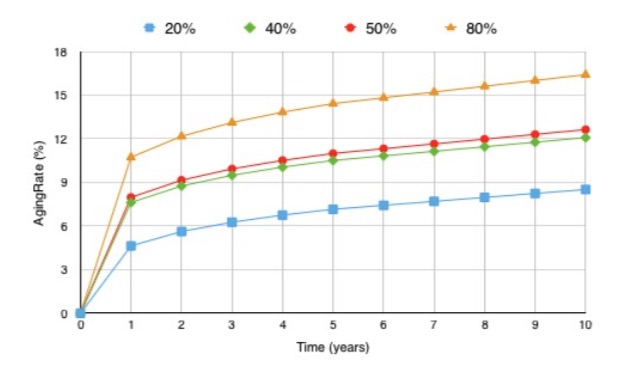
\includegraphics[width=0.9\columnwidth]{agr.png}
	\caption{aging rates of buffers with different clock duty cycles}
	\label{fig:agr}
\end{figure}
\begin{figure}
	\centering
	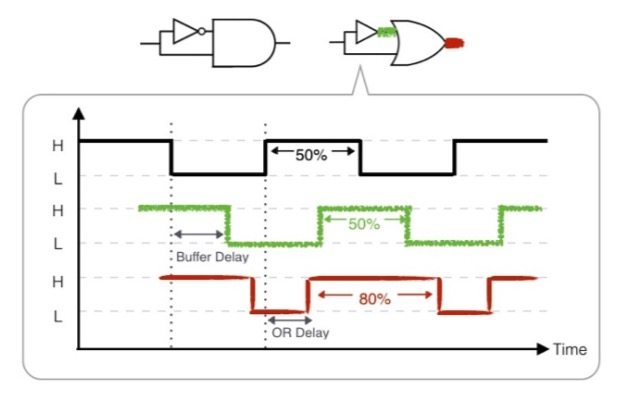
\includegraphics[width=0.9\columnwidth]{dcc.png}
	\caption{Construction of DCC and duty-cycle transformation}
	\label{fig:dcc}
\end{figure}
\begin{figure}
	\centering
	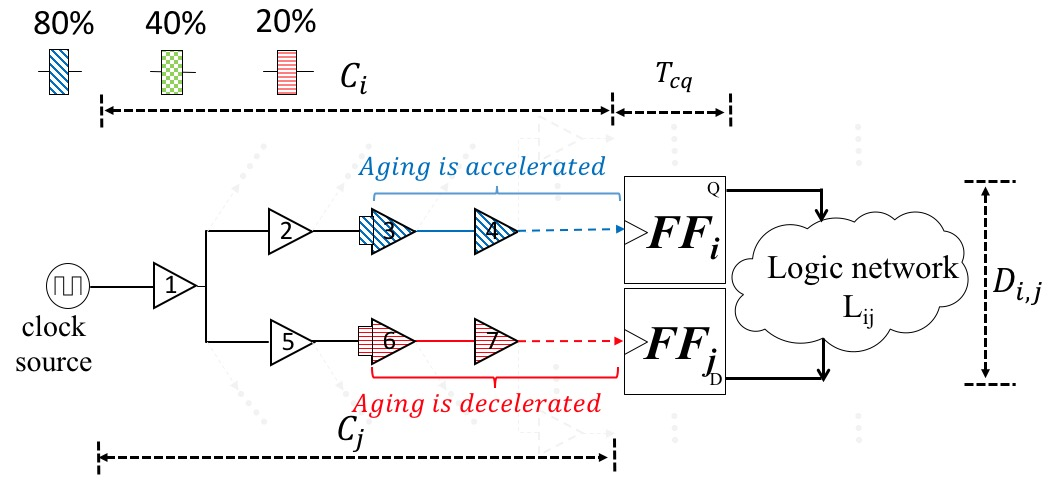
\includegraphics[width=0.9\columnwidth]{exp.png}
	\caption{Example of DCC insertion}
	\label{fig:exp}
\end{figure}

\subsection{Duty-Cycle Converter (DCC)}
Duty cycle is the percentage of one period in which a signal is high (i.e., logic 1). We have known that the aging of logic gates highly depends on the stress time [8]. For a clock buffer on the clock tree, its stress time is proportional to the clock duty cycle. Therefore, by adjusting the clock duty cycle, we can manipulate the aging of clock buffers and then control the effective degradation of logic paths. \ref{fig:agr} shows the aging rates of clock buffers with different clock duty cycles.
The unit we use to change the clock duty cycle is duty-cycle converter (DCC). A DCC includes an inverter/buffer and an AND/OR gate. It can convert the duty cycle of a clock signal to a smaller/larger one. \ref{fig:dcc} shows a DCC and the conversion of the clock duty cycle from 50\% to 80\%. It separates the source clock wave (black line) to a delayed wave (green line, may be inverted) and original wave. Then, those two waves are combined with the OR gate to obtain a new clock wave (red line) of 80\% duty cycle.
\subsection{DCCs against a Critical Path}
Once we insert a DCC into the clock tree, the downstream sub-tree of the DCC insertion point will receive a clock signal whose duty cycle is no longer 50\%. Consider the circuit in \ref{fig:exp}: we insert an 80\% DCC on the left clock path to accelerate its aging and a 20\% DCC on the right clock path to decelerate its aging. Over several years, the left clock latency will gain greater than the right one does. Therefore, setup-time violations are likely to occur on this critical path.